\chapter{Evaluación}
\label{chap:evaluation}
\label{chap:5}

\section{Evaluación de mejoras}

\subsection{Evaluación BVH}
	
En el \autoref{chap:4} se ha hablado de la implementación de árboles BVH, pero no se ha mostrado ninguna comparativa sobre que ventajas ofrece frente al método ingenuo. Por esta razón, se han evaluado tres escenas, de número de triángulos creciente, sin y con la mejora. El resultado ha sido el esperado: para escenas de muchos triángulos, la diferencia es órdenes de magnitud más eficiente. La complejidad del método ingenuo crece linealmente con el número de triángulos, de manera que deja de ser viable utilizarla en el momento en el que las geometrías se complican.\\

\begin{tabular}{ |p{3cm}||p{3cm}|p{3cm}|p{3cm}| }
	 \hline
	 \multicolumn{4}{|c|}{Accelerator structure BVH comparaison} \\
	 \hline
	 Model Name&No BVH&BVH&Speedup\\
	 \hline
	 Suzanne   &8357 kPath/s&13973 kPath/s&167.20\%\\
	 Stanford Bunny &1806 kPath/s&13960 kPath/s&772.97\%\\
	 Stanford Dragon &14 kPath/s &11507 kPath/s&82192.85\%\\
	 \hline
\end{tabular}

\subsection{Selección de parámetros BVH}
	
Finalmente es necesario elegir los parámetros para \code{BVH\_DEPTH} y \code{SAH\_BINS}. Puesto que existen varios tipos de escenas con distintas geometrías, se va a dejar de lado cualquier tipo de enfoque analítico y se va a hacer uso de medidas en casos reales. Se procede a realizar una evaluación con distintos parámetros.
	
En el caso de la selección de \code{SAH\_BINS}, Indigo Wald propone 16 como límite \cite{wald2007fast} debido a la insustancial mejora de rendimiento para valores mayores. Esto se ha podido comprobar directamente en Eleven Renderer donde se ha llevado a cabo la construcción y recorrido de BVH para la escena "Stanford Dragon" variando la cantidad de contenedores \autoref{fig:sahbins}. Se comprueba que la velocidad de recorrido se estanca para los valores 12-16, mientras que el tiempo de generación permanece lineal. Eleven Render utiliza de manera predeterminada \code{SAH\_BINS = 14} tras el análisis realizado.

\begin{figure}[H]
\centering
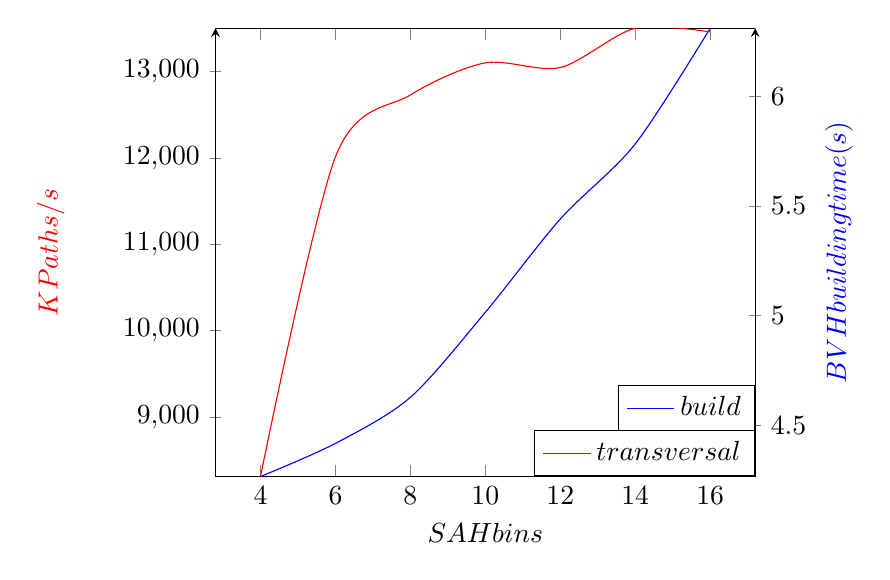
\begin{tikzpicture}

\begin{axis}[
    axis y line = right,
    xlabel = \(SAH bins\),
    ylabel = {\(\textcolor{blue}{BVH building time (s)}\)},
	legend style={at={(1,0.1)},anchor=south east},
	scaled y ticks=false
]

\addplot[smooth, blue]
coordinates{(4,4.267) (6, 4.418) (8, 4.628) (10, 5.015) (12, 5.440) (14, 5.782) (16, 6.309)};
\addlegendentry{\(build\)}
\end{axis}

\begin{axis}[
    axis y line = left,
	axis x line = none,
    xlabel = \(SAH bins\),
    ylabel = {\(\textcolor{red}{KPaths/s}\)},
	ylabel style={yshift=0.5cm},
	legend style={at={(1,0)},anchor=south east},
	scaled y ticks=false
]

\addplot [smooth, red]
coordinates{(4,8310) (6, 12012) (8, 12728) (10, 13100) (12, 13046) (14, 13501) (16, 13458)};
\addlegendentry{\(transversal\)}

\end{axis}
\end{tikzpicture}
\caption{Comparación de tiempos de construcción y eficiencia de recorrido para distinto número de contenedores}
\label{fig:sahbins}
\end{figure}


\section{Evaluación Nsight Compute}

Para llevar a cabo la evaluación del algoritmo se ha hecho uso de la herramienta NVIDIA Nsight Compute. Esta herramienta proporciona un análisis completo sobre la ejecución de un kernel, así como información relevante que puede dar pistas de dónde están los cuellos de botella y que partes conviene optimizar.

Tras crear un proyecto y acceder al perfil de \code{renderingKernel}, el primer dato de relevancia que se ha buscado ha sido que parte del código es la más ejecutada. Conociendo este detalle se puede evitar el esfuerzo de optimizar partes poco relevantes. Para conocer este dato es necesario acceder a la pestaña \code{Source} de la aplicación. En esta pestaña se visualiza el código junto a las instrucciones pptx y a la derecha un mapa de calor que indica en qué partes del código frecuentan más los filtros seleccionados en la pestaña \code{Navigation}.

Se ha seleccionado el filtro de instrucciones ejecutadas donde se han podido localizar dos principales puntos calientes. El primero de los dos es el acceso a los hijos en los nodos del árbol BVH. El segundo es en las funciones de mínimo y máximo. Esto es de esperar ya que son funciones aritméticas que se utilizan en el cálculo de la intersección del rayo con los nodos del árbol.

\begin{figure}[H]
    \centering
	\includegraphics[width=0.5\textwidth]{instructionsexecutedbvh}
	\caption{Nº instrucciones ejecutadas funciones leftChild, rightChild}
	\label{fig:label}
\end{figure}

\begin{figure}[H]
    \centering
	\includegraphics[width=0.5\textwidth]{instructionsexecutedminmax}
	\caption{Nº instrucciones ejecutadas funciones minf/maxf}
	\label{fig:label}
\end{figure}

Estos resultados muestran que la mayoría de las instrucciones ejecutadas se encuentran en el recorrido de los árboles BVH. No es de extrañar que la mayoría de los esfuerzos de optimización del trazado de rayos en el estado del arte residan en estructuras de aceleración más óptimas y compactas. 

NVIDIA Nsight Compute también ofrece advertencias de que partes pueden resultar problemáticas o subóptimas en una arquitectura de GPU en el panel \code{Details}. La ejecución de Eleven Renderer provoca el aviso de un error común en arquitecturas paralelas y es el acceso no secuencial de la memoria. Este fenómeno ocurre cuando los hilos de un wrap no acceden a posiciones contiguas, y en el caso de esta evaluación la advertencia redirige a la parte del código que accede a los hijos del árbol BVH. Esto es de esperar puesto que las estructuras de los árboles no ofrecen buena secuencialidad.

\begin{figure}[H]
    \centering
	\includegraphics[width=0.7\textwidth]{memoryaccess}
	\caption{Advertencias de acceso no secuencial}
	\label{fig:label}
\end{figure}


\subsection{Análisis Roofline}
	
El modelo Roofline es utilizado en el análisis de eficiencia de aplicaciones de altas prestaciones. Es un modelo que simplifica la visión del hardware y software mostrando un posible techo de eficiencia. NVIDIA Nsight Compute ofrece este análisis para poder analizar posibles deficiencias y optimizaciones.

La línea superior es una cota superior de 29.23 TFLOPS

El análisis de ejecución de Eleven Renderer para precisión simple \autoref{fig:roofline} ha resultado en 0.36 FLOP/byte de intensidad aritmética y 124.47 GFLOPS de eficiencia, mientras que el techo para una intensidad aritmética de 0.36 FLOP/byte está en 330.65 GFLOPS. Esto indica que el algoritmo está corriendo a un 37.6\% de su capacidad máxima teórica según este modelo siempre y cuando la intensidad aritmética no varíe. Este resultado es razonable, indica que no se está infrautilizando el acelerador gráfico, además indica que el algoritmo tiene una gran dependencia de memoria al encontrarse el punto ubicado a la izquierda.

Si se quisiera optimizar más aún este motor, un buen camino sería romper esta dependencia.

\begin{figure}[H]
    \centering
	\includegraphics[width=0.9\textwidth]{roofline}
	\caption{Análisis Roofline}
	\label{fig:roofline}
\end{figure}


